%----------------------------------------------------------------------------------------
%	DOCUMENT CONFIGURATIONS
%----------------------------------------------------------------------------------------

\documentclass[a4paper,11pt]{report}
\usepackage[francais]{babel}
\usepackage[utf8]{inputenc}
\usepackage[T1]{fontenc}
\usepackage{ucs}
\usepackage{url}
\usepackage{graphicx}
\usepackage[table]{xcolor}
\usepackage{mathtools,amssymb,amsthm}%
\usepackage[left=2.5cm,top=2cm,right=2.5cm,nohead,nofoot]{geometry}
\usepackage{float}
\linespread{1.1}

\begin{document}


\setlength\parindent{0pt} % Removes all indentation from paragraphs


\begin{titlepage}
\begin{center}
\textbf{\textsc{UNIVERSIT\'E LIBRE DE BRUXELLES}}\\
\textbf{\textsc{Faculté des Sciences}}\\
\textbf{\textsc{Département d'Informatique}}
\vfill{}\vfill{}
\begin{center}{\Huge Analyse vidéo pour la détection, \\ suivi et reconnaissance de poissons}\end{center}{\Huge \par}
\begin{center}{\large \textsc{Della Monica} Simon, \textsc{Ooms} Aurélien, \textsc{Sonnet} Jean-Baptiste}\end{center}{\Huge \par}
\vfill{}\vfill{}
\begin{flushleft}{\large \textbf{Superviseur : Yann-A\"{e}l Le Borgne}}\hfill{}\end{flushleft}{\large\par}
\vfill{}\vfill{}\enlargethispage{3cm}
\textbf{Année académique 2012~-~2013}
\end{center}
\end{titlepage}




\tableofcontents
\newpage

\chapter{Introduction}

%----------------------------------------------------------------------------------------
%	Introduction
%----------------------------------------------------------------------------------------

\section{Motivation}

L'analyse logicielle vient de plus en plus appuyer le travail de ceux pour qui la récolte d'informations provient essentiellement d'une source numérique, i.e des vidéos enregistrées lors d'observations menées par des biologistes ou statisticiens, etc.
 
L'usage de procédés automatisés permet le filtrage et l'analyse massive de données qui était jusqu'alors une tâche fastidieuse à traiter. Données qui une fois traitées permettent d'inférer ou d'appuyer des thèses selon les besoins.

Par exemple, l'analyse des déplacements individuels au sein d'un banc de poissons filmé pendant un longue période est une tâche pour laquelle le passage par un traitement informatisé apparaît comme nécessaire.\\

Le but de ce projet est d'ébaucher une solution logicielle d'analyse vidéo permettant l'automatisation du travail de détection et de suivi de poissons dans un milieu donné. 

\section{Approche et solution}
Dans le cadre de ce projet, l'algorithme \textit{condensation} a été implémenté comme solution pour le suivi de cibles.

La réalisation de l'application comprenait plusieurs étapes:
\begin{enumerate}
\item Segmentation
\item Détection de traits d'intérêts 
\item Observations
\item Prédictions
\item Évaluation et Mise en correspondance
\end{enumerate}
Chacune de ces étapes a nécessité la compréhension de ses enjeux et des différentes réponses qui y ont été apportés. Suite à quoi, une implémentation a été choisie pour chacune d'elles.
La concaténation de ces étapes a abouti en une implémentation de l'algorithme \textit{condensation}.\\

Dans la recherche de solutions, d'autres approches ont été explorées, particulièrement l'algorithme SURF. Ce dernier sera exposé dans la section éponyme.  

%----------------------------------------------------------------------------------------
%	SECTION 2
%----------------------------------------------------------------------------------------

\chapter{\'{E}tat de l'art}

Il existe un grand nombre d'approche pour traiter la détection et le suivi d'objet au travers de flux d'images. 

Il est nécessaire de prendre connaissance de ces différentes approches et leur évolution, ainsi que des bénéfices ou contraintes qu'elles induisent. D'autre part le sujet étant prolixe, nous limiterons ici l'exposé des méthodes de détection et de suivi à celles que nous avons utilisée ou celles qui nous sont, à un moment ou l'autre, apparues importantes pour traiter de la problématique qui nous occupe.

\section{Contexte, matériaux et questions}
Une vidéo est un flux, une succession d'images, dites  \textit{frames}. Le flux est dépendant de la fréquence de lecture/d'affichage, soit un taux en fps (\textit{frames per second}). 

Suivre une cible au long d'une séquence d'images, c'est définir et reconnaître une partie de l'image courante comme identique à la précédente, tout en lui autorisant des modifications (taille, position, couleur,...). Rétroactivement, c'est aussi reconstruire la trajectoire d'une cible dans la séquence d'images, cette approche se montrera pertinente pour la suite.\\

Le \textit{video tracking} ou suivi de cibles au sein d'une vidéo est le suivi de morceaux ciblés d'images au travers du flux duquel elles proviennent. C'est la tâche automatisée qui consiste en la localisation, d'images en images, d'un groupe de pixels généralement en mouvement. \\

Si une cible apparait à l'oeil humain comme consistante alors qu'elle se meut dans son champs de vision, il en va tout autrement en \textit{computer vision}. En effet, à tout instant la consistance conférant son unité à la cible doit être déterminée, calculée et éprouvée pour qu'elle soit reconnue. 

Les parties traquées sont en fait chacune une quantité donnée de pixels, dans une espace restreint. Quantité à laquelle on concédera une identité en lui définissant/reconnaissant des attributs propres (variants et invariants). La cible sera alors contenue dans une \textit{région d'intérêt}, c'est-à-dire une sous-matrice d'une matrice plus grande que représente l'image toute entière.\\

\begin{figure}[hbtp]
\centering
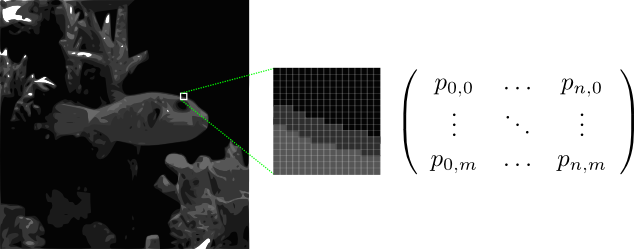
\includegraphics[scale=1]{figureImageMatrice.png}
\caption{Matrice de pixels}
\end{figure}


On perçoit plusieurs difficultés qu'il conviendra de maîtriser: l'unité de la cible et sa différenciation du fond, l'identité de celle-ci, malgré des modifications intrinsèques dans le flux d'images, la caractérisation et détermination du mouvement de la cible.\\
Deux problématiques fortement liées peuvent être dégagées\footnote{Video Tracking: A Concise Survey, E. Trucco, K. Plakas, IEEE Journal of Oceanic Engineering, Avril 2006}: le \textit{mouvement} et la \textit{correspondance}.

\subsection{La question du \textit{mouvement}}

	La question du mouvement comporte deux aspects: la détermination d'une cible comme mouvante et la caractérisation de ce mouvement.
	
\subsubsection{Une cible mouvante}	
	L'approche qui semble la plus évidente pour cerner une cible en mouvement est sa différenciation avec ce qui apparait comme statique. 
	
	On supposera les objets d'intérêt et mouvant, comme appartenant à l'avant-plan (\textit{foreground}) et le reste, statique, comme appartenant au fond (\textit{background}). On parlera alors de \textit{soustraction du fond}.

\[F(\lambda_t) = \lambda_t - B_t\]	
où,
\begin{itemize}
\item[] $\lambda_t$ est une frame à l'instant $t$
\item[] Le \textit{foreground}: $F(\lambda_t)$ 
\item[] La \textit{background}, la matrice $B_t$\\
\end{itemize}

	La soustraction du fond peut se réaliser de différentes manières, mais elle doit pouvoir résister aux changements de luminosité, aux bruits et aux différentes variations de vitesse.
	De façon générale, l'extraction s'obtient en soustrayant de l'image courante une image de "référence", le fond.
	L'image de référence est actualisé à chaque étape, par accumulation pondérée et relativement à l'avant-plan extrait:
	
	$$\texttt{dst}(x,y)  \leftarrow (1- \alpha )  \cdot \texttt{dst}(x,y)+\alpha \cdot \texttt{src}(x,y)$$
	$$\texttt{if} \quad \texttt{mask} (x,y)  \ne 0$$
	où,	
	\begin{itemize}
	\item[] $\alpha$ est le \textit{facteur d'oubli}
	\item[] $\texttt{dst}(x,y)$ est le pixels de destination et $\texttt{src}(x,y)$ celui de l'image source.
	\item[] $\texttt{mask} (x,y)$ est une image binaire générée à partir de l'avant-plan extrait en $t-1$.
	\end{itemize}


\subsubsection{Un mouvement déterminé}		
	Le mouvement est caractérisé par une position d'origine (vecteur position), une direction (orientation vers un point de destination relativement a un référentiel) et une vitesse (obtenu en dérivant les coordonnées par rapport au temps).	
	L'enjeu est de parvenir déterminer que la position d'une cible à un instant $t$ est la résultante d'un mouvement, de cette même cible, initié en $t-1$.\\
	
	Plusieurs approche sont envisageables, notamment la définition du mouvement d'image de J.Shi et C.Tomasi .
	
	Le \textit{mouvement d'image}:
	$$I(x,y,t+\tau)=I(x-\xi(x,y,t,\tau),y-\eta(x,y,t,\tau))$$
	où
	\begin{itemize}
	\item[] $I_{t+\tau}$ est une image obtenue à partir d'un déplacement des points à l'instant $t$.
	\item[] Le vecteur de \textit{déplacement} $\delta = (\xi,\eta)$ est la quantité de mouvement. On perçoit l'insuffisance de la définition du déplacement $\delta$ quant aux multiples déplacements internes à la cible.\\
	\end{itemize}
	Le déplacement comme \textit{champs de mouvement affine}:
	$$\delta = D\texttt{x}+\texttt{d}$$
	où
	$D$ est la matrice de déformation et $d$ une translation sont donné comme:
	$$ D = \left( 
		\begin{array}{cc}
		d_{xx} & d_{xy} \\
		d_{yx} & d_{yy} \\ 
		\end{array} 
		   \right)
	$$
	Ce qui permet de poser pour un point $x$, centre d'une région d'intérêt de l'image $J_t$ son mouvement équivaudra au point $Ax + \texttt{d}$ de l'image suivante $J_{t+\tau}$, où $A = I + \texttt{D}$ et $I$ est la matrice identité donnée par:$$J_{t+\tau}(Ax + \texttt{d}) = J_t(x)$$\\
	La prédiction du mouvement sera donnée par l'estimation des paramètres de la matrice $D$ et du vecteur de déplacement $\texttt{d}$.\\
	
	
	
	Un autre approche plus courante est celle s'appuyant sur le concept de flux optique dont l'introduction est attribuée au psychologue James J. Gibson\footnote{\url{http://fr.wikipedia.org/wiki/Flux_optique}} . 
	
	Le flux optique (\textit{Optical Flow}) est décrit comme le modèle sous-jacent au mouvement visible d'un objet dans son contexte et relativement à l'observateur. Ce mouvement peut être estimé à partir d'une séquence d'images comme une suite de vitesses instantanées ou de déplacements discrets d'images.\\ 
	
	%l'une serait de cerner une région (autour de la cible) qui aurait une probabilité acceptable de contenir la cible à l'image suivante. La taille de la région serait donnée en fonction d'un mouvement prévu/attendu calculé sur une estimation précédente. Ce qui reviendrait à prédire et identifier une région dans laquelle l'élément ciblé aurait la plus grande probabilité de se trouver à l'image suivante. 
	
	%Estimer cette région à forte probabilité pourrait s'obtenir par le calcul de positions futures acceptables, pour chaque pixel définissant la cible (en prenant en compte l'historique récent de leurs mouvements).\\
	%Toutefois ce procédé semble rencontrer des difficultés d'une part lorsque la vitesse de la cible est sensiblement plus grande que le taux de frames du flux vidéo et d'autre part, lorsque la cible est de couleur relativement uniforme. Pour cerner le déplacement d'un pixel, il faut être en mesure de différencier la destination des attributs propres à l'origine et donc au pixel en mouvement, d'une façon certaine l'apparence uniforme empêche de faire apparaître les pixels comme mouvant, car la différenciation semble compromise. En ne focalisant plus sur un pixels, mais sur un groupes de pixels, la différenciation devient plus aisée, mais au détriment d'une sensibilité certaine et d'une définition précise du contour. C'est la problématique de l'ouverture, des block plus grands apparaissent plus sur et sont d'ailleurs moins sensible au bruit, mais offre moins de précisions\footnote{Block Matching for Object Tracking, A.Gyaourova, C.Kamath, S.C. Cheung, Department of Computer Science, University of Nevada, Reno, Center for Applied and Scientific Computing Lawrence Livermore National Laboratory, 2003}. \\
	% Un autre approche qui fait consensus est l'utilisation du \textit{filtre Kalman}\footnote{
%P. S.Maybeck, Stochastic Models, Estimation and Control. London U.K. Academic, 1979, vol. 1,2.}, celle-ci se révèle beaucoup plus performante.  

\subsection{La question de la \textit{correspondance}}

L'objectif est de reconnaître et identifier une cible d'une frame à l'autre. 

\subsubsection{Critères d'intérêt}
Pour suivre une cible, on la compare au travers du flux d'images selon certaines \textit{unités de mesure}.
Ces unités de mesure sont façonnées au regard de la problématique traitée. Elles peuvent \^etre complexes et sont généralement hautement dépendantes des paramètres qui les composent.

Une unité de mesure est un ensemble des caractéristiques paramétrant l'objet cible, telles la position du centre de masse, l'aire, les coins, les contours ou encore l'historique des mouvements antérieurs. \\

La paramétrisation de la cible est capitale, car elle doit offrir des garanties sur l'identité de l'objet traqué. 
D'une image à l'autre, on doit pouvoir s'appuyer sur des critères robustes à l'évolution de la cible dans le flux d'image.


Il faut trouver des caractéristiques présentant des propriétés locales remarquables, c'est-à-dire des traits d'intérêts, stables ou \textit{invariants}, on parlera de \textit{features} de la cible.

Il existe diverses méthodes de détection de zones d'intérêts, chacune relative aux types de zones d'intérêts sur lesquels on souhaite baser l'analyse de la cible. Citons parmi les plus connu, l'algorithme de détection de coins de C. Harris et M. Stephens ou encore celui de J. Shi et C. Tomasi sur l'estimation qualitative des traits d'intérêts, mais aussi l'algorithme de détection de contours, \textit{Canny edge detection}, présenté par l'australien J. Canny en 1986.

\subsubsection{Fonction de mérite}
Une fois la caractérisation choisie, il faut établir une méthode de comparaison débouchant sur un coefficient de qualité sanctionnant l'estimation ou la prédiction de correspondance.\\

Une fonction de mérite, \textit{figure-of-merit}, est une fonction qui mesure la concordance entre les données et le \textit{modèle}, tout en considérant un choix particulier de paramètres.\\

En statistique fréquentielle, la fonction de mérite est généralement agencée de sorte que de petites valeurs obtenues représentent une concordance étroite. Tandis qu'une approche bayésienne choisirait une fonction de mérite de sorte à ce que des valeurs élevées représentent une meilleure concordance \cite{n}.

La fonction de mérite devra être telle qu'elle offre la meilleur façon de trouver l'extremum désiré en fonction des caractéristiques prédéfinies de la cible.\\

Elle devra aussi considérer que les données récoltées sont généralement bruitées.
Du fait que l'objet cible se modifie tout au long du flux d'images, la reconnaissance des critères comme correspondant comprend aussi leur différenciation du contexte/bruit. 

Par exemple, l'environnement où évolue la cible pourrait présenter l'une ou l'autre parcelle d'images assez ressemblante que pour passer comme identique au regard de l'unité de mesure définie.
De façon générale, pour outrepasser la pollution issue d'éléments parasites valides, il sera souvent nécessaire de mettre en œuvre plusieurs approches.
% existe des techniques de \textit{filtrage}, tel l'algorithme \textit{Conditional Density Propagation} \footnote{ Michael Isard and Andrew Blake, Int. J. Computer Vision, 29, 1, 5--28, (1998).
%$http://homepages.inf.ed.ac.uk/rbf/CVonline/LOCAL\_COPIES/ISARD1/condensation.html$ } ou d'isolation de la cible avec la méthode \textit{Gap-Mountain}\footnote{Moving Object Tracking in Video, Yiwei Wang and John Doherty and Robert Van Dyck, Department of Electrical Engineering, The Pennsylvania State University, National Institute of Standards and Technology}. 
%Ces techniques de filtrage de particules permettent aussi le tracking d'éléments dont le nombre varie au fil du temps \footnote{Filter-based Predictive Tracking for Robust Fish Counting, E. Morais, M. Campos, F. Pádua, R. Carceroni
%UFMG–Universidade Federal de Minas Gerais, Belo Horizonte, MG, Brasil} .

%\subsection{Problématique de l'identification}
%Le dénombrement et la classification des cibles peut être une démarche très utile. Par exemple, comptage des individus dans les fermes d’élevage ou classification des espèces en pleine nature, ou encore étude des relations prédateur-proie\footnote{One Fish, Two Fish, Butterfish,Trumpeter : Recognizing Fish in Underwater Video}.\\
%Techniquement, il est difficile de différencier des espèces de poissons en se basant uniquement sur une vidéo. En effet, plusieurs facteurs sont à prendre en compte :
%\begin{itemize}
%\item Déformations
%\item Décalage des couleurs
%\item Sédiments parasitant la visibilité
%\item Luminosité variable\\ 
%\end{itemize}
%
%Différents facteurs sont à prendre en compte lors de la tentative de reconnaissance :
%\begin{itemize}
%\item la cible peut apparaître de différentes manières devant l’objectif.\\ Pour résoudre ce problème, on utilise un algorithme de transposition au sein duquel on essaiera de faire correspondre la forme du poisson à , en tenant compte des différentes déformations.
%\item La déformation due à la distance par rapport à l’objectif.
%\end{itemize}
\subsection{Luma, luminance et niveau de gris}
La plupart des algorithmes de traitement d'images fonctionnent à partir d'images couleurs transformées en niveau de gris, c'est-à-dire ne considérant que l'intensité lumineuse de l'image.\\
 
La lumière dénuée de couleurs est dite monochromatique ou achromatique. L'unique attribut d'une telle lumière est son intensité. L'image en \textit{niveau de gris} représente alors l'intensité achromatique de l'image.\\ 

D'une image en niveau de gris, on peut d'une part travailler sur l'intensité des objets décrits dans l'image, et d'autre part réduire le coût computationnel du traitement en ne considérant qu'une valeur par pixels.\\

La luminance est définie de différentes façons, ce qui peut porter à confusion. Globalement, la luminance, définie en \textit{lumens}, mesure la quantité d'énergie qu'un observateur perçoit d'une source de lumière donnée.  
\subsubsection{Luma ou luminance}
On parlera de luma pour décrire la luminance calculée d'un appareil visuel et de luminance lorsqu'il s'agit de la grandeur physique ou de la luminance relative.
Les deux termes désignent un même phénomène physique, leur distinction provient de l'usage qui en est fait.
 
\begin{enumerate}
\item Luma est utilisé dans le domaine vidéo. C'est la brillance de l'image, soit la partie du signal vidéo correspondant à l'intensité lumineuse.  

Elle représente donc la part achromatique de la vidéo, mais précisément la "quantité de lumière" présente dans l'image résultante de l'application de la loi de puissance \textit{gamma}.\\

\item La luminance relative, est l'intensité de l'image calculée selon un espace colorimétrique précis, cette appellation est couramment utilisée en imagerie numérique.\\
\end{enumerate}

Dans le domaine vidéo, gamma est le facteur qui caractérise le contraste d'un signal visuel. C'est une relation qui approche une loi de puissance liant amplitude de la luminance du signal et luminance réelle de l'image à l'écran. 

Ce facteur était initialement dû au fait que les tubes cathodiques avaient une courbe de réponses qui ne réagissait peu ou pas pour des amplitudes de signal trop faible. Le facteur gamma était alors calculé tel qu'il corrigeait le problème. 

Le facteur gamma est utilisé pour la calibration du support d'affichage des images afin que celle-ci apparaissent normale à l'œil humain.\\

La luminance relative et la valeur luma sont calculées identiquement comme une somme pondérée des composantes RGB et suivant le cas après \textit{correction gamma} des images vidéos ou pas:
$$ Y' = 0.299*R' + 0.587*G' + 0.114*B' $$
où
\begin{description}
\item[$Y'$] est la valeur de luma.
\item[$R'$,$G'$,$B'$] sont les composantes RGB après correction gamma.\\
\end{description}

Les coefficients permettent de se rapprocher au mieux de la perception humaine des couleurs. On voit en particulier que, dans la perception humaine de l'intensité lumineuse, le vert intervient sensiblement plus, contrairement au bleu.

Ces coefficients sont déterminés relativement au support d'affichage et sont précisés dans des recommandations. 

Les plus courantes sont:
\begin{enumerate}
\item la recommandation Rec. 709 pour les HDTV donne pour luma: 
$$Y =  0.2126*R+0.7152*G+0.0722*B $$ 
\item la recommandation CCIR 601 donne pour luma: 
$$Y =  0.299*R+0.587*G+0.114*B $$
\end{enumerate}
Ces recommandations sont faites de telle façons que les couleurs fondamentales et le blanc soient correctes et donc que la représentation de la luminance soit maintenue.\\


\subsubsection*{Niveau de gris}

L'image en niveau de gris est obtenue en attribuant aux composantes de chaque pixel la valeur en luma ou luminance de ce point.
$$
	\forall p \in I_{m*n}, \left\{
	\begin{array}{l l}
	Y'_p = 0.299*R'_p + 0.587*G_p' + 0.114*B'_p \\ 
	p_{[r,g,b]} = [Y'_p,Y'_p,Y'_p] 
	\end{array} \right.
$$


Une autre approche plus simpliste est de calculer le niveau de gris d'un pixels $p$ à partir de sa coloration moyenne: \[p_{\{r,g,b\}} =\frac{p_r+p_g+p_b}{3}\]

\pagebreak
%%%%%%%%%%%%%%%%%%%%%%%%%%%%%%%%%%%%%%%%%%
\section{Caneva}
Même s'il n'est pas de structure commune aux algorithmes existants pour la détection et le suivi de cible en mouvement, les étapes suivantes semble prévaloir pour beaucoup de ceux-ci.\\
\begin{center}
\begin{tabular}{ c c c c c c c } 
\cellcolor[gray]{0.9} Segmentation & $\rightarrow$ & \cellcolor[gray]{0.9} Extraction & $\rightarrow$ & \cellcolor[gray]{0.9} Analyse & $\rightarrow$ & \cellcolor[gray]{0.9} Suivi\\  
\end{tabular} 
\end{center}

\subsection{Segmentation}
A cette étape, il s'agit de dégrossir le matériau brut, de simplifier l'image en ne gardant que ce qui fait sens pour les opérations suivantes. L'objectif sous-tendant à toutes méthodes de traitement d'images étant de minimiser l'usage inutile de ressources computationnelles, la segmentation de l'image est une première approche pour ne plus focaliser que sur le signifiant. 

La segmentation est une opération de partitionnement de l'image en un certain nombre de segments. Cette opération est utilisée pour dégager des zones d'intérêts de l'image. Elle assigne une étiquette à chaque pixel de sorte que tous pixels identiquement étiquetés partagent des caractéristiques visuelles données (couleur, intensité, texture). Aussi tous les segments adjacents sont sensiblement différents suivant ces caractéristiques \footnote{\url{http://en.wikipedia.org/wiki/Segmentation_(image_processing)}}.\\

Il existe différentes méthodes de segmentation, certaines travaillent sur base de régions qu'elles accroissent, décomposent ou fusionnent, d'autres sur les contours, la classification ou le seuillage des pixels en fonction de leur intensité.

\subsubsection{Image binaire}
La méthode de segmentation la plus simple et la plus rapide est la création d'une image monochrome (aussi appelée \textit{binaire}) par seuillage: \`A partir de l'image originale convertie en niveaux de gris, on la transforme comparativement à une valeur seuil prédéterminée en une image binaire où chaque pixel prendra une des deux valeurs possibles.\\

La transformation suivra la règle suivante:\\
soit une image $I$ de taille $m*n$, un seuil $T$ \textit{global} et $g(x,y)$ le niveau de gris du point $(x,y)$,

$$ \forall (x,y) \in I_{\{m,n\}}, (x,y) = \left\{ 
\begin{array}{rl}
1 &\mbox{si } g(x,y)>T\\
0 &\mbox{sinon}
\end{array} \right.
$$ 
Où les pixels appartenant à un objet de l'avant-plan sont étiquetés $1$ et ceux provenant du fond sont étiquetés $0$.\\ 

Cette approche grossière de seuillage peut être affinée par l'usage d'un histogramme de niveau de gris, offrant notamment la possibilité de segmenter l'image selon de multiples seuils.

Ou encore, plutôt que d'utiliser un seuil \textit{global}, il est possible de faire dépendre $T$ de propriétés locales du point évalué, comme par exemple de la valeur moyenne du niveau de gris de l'entourage du point considéré. On parlera d'un seuillage \textit{adaptatif} ou \textit{dynamique}.\\

L'image binaire peut, ensuite, être utilisée comme un masque permettant d'isoler des régions potentiellement intéressantes.

\subsubsection{Watershed}
L'algorithme de segmentation \textit{Watershed}, traduit par "ligne de partage des eaux", se base sur une interprétation tridimensionnelle de l'image, où un point est caractérisé par ses deux composantes spatiales et son niveau de gris.

De cette image, perçue comme un relief topographique, sera calculée la ligne de partage des eaux pour délimiter le bassin-versant, c'est-à-dire l'aire à l'intérieur de laquelle convergerait de l'eau hypothétiquement tombée. 

Trois types de points sont définis par cette interprétation:
\begin{itemize}
\item ceux appartenant à un minimum local.
\item ceux à partir desquels une goutte d'eau s'écoulerait inévitablement vers une minimum local précis. L'ensemble des points relatés à un même minimum constitueront un bassin-versant de ce minimum.
\item ceux à partir desquels toute goutte d'eau ruissellerait équitablement vers l'un ou l'autre minimum. L'ensemble des ces points forment topologiquement une crête, ils constituent la ligne de partage des eaux.\\
\end{itemize} 
 

Il existe plusieurs d'implémenter cet algorithme, parmi les plus communes: 
\begin{itemize}
\item selon la distance topographique d'un point au minimum le plus proche, à partir de chaque pixel de l'image, on suit le gradient jusqu'à atteindre un minimum, à l'image d'un ruissellement.
\item par inondation, où est simulé une montée progressive du niveau d'eau à partir des minima du relief.\\
\end{itemize}

La segmentation par ligne de partage des eaux donne de bons résultats dans l'extraction d'objet presque uniforme, mais conduit souvent à une sur-segmentation dû aux bruits et irrégularités locales. Une façon de pallier à ce désavantage est d'utiliser des marqueurs. Les marqueurs sont définis comme des composantes connexes appartenant soit à un objet d'avant-plan, soit au fond. La sélection des marqueurs à garder pourra être effectuée par simple estimation du niveau de gris et de la connectivité.%   


\subsubsection{Détection de contours}
Intuitivement, un contour est défini comme une suite de pixels contigus reflétant la frontière entre deux régions. 
La détection des contours permet alors de découper ou fusionner l'image en sous-régions.

En pratique, les principaux algorithmes de détection de contours, \textit{edge detection}, se basent sur l'étude des dérivées de la fonction d'intensité de l'image: le gradient, les extremums locaux et le passage par zéro du Laplacien. Le contour est obtenu par détection d'une discontinuité (changement abrupte d'intensité) et des similarités (selon des critères prédéfinis).\\

\begin{figure}[hbtp]
\centering
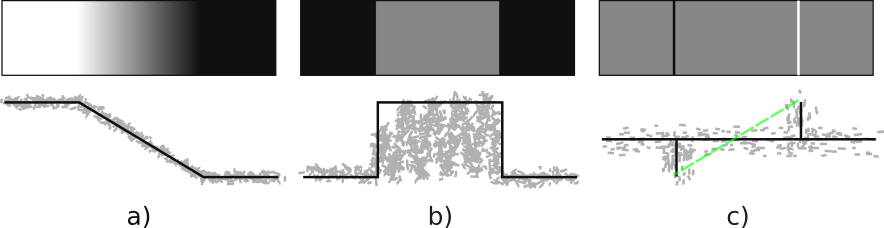
\includegraphics[scale=0.6]{figureDetectionDiscontinuities.png}
\caption{Détection de contours}
\label{fig:DetectionDiscontinuities}
\end{figure}

Dû notamment aux différentes méthodes d'acquisition, la frontière entre deux régions n'est pas toujours très contrastée ni exempte d'aucun bruit. De fait, elle apparaîtra généralement floutée et bruitée.\\ 
\`A partir d'une image en niveaux de gris, la frontière d'une région à une autre, représenté en \textit{a} dans la figure \ref{fig:DetectionDiscontinuities}, peut être \textit{idéalement} définie par une fonction rampe dont la longueur sera caractérisé comme le niveau de floutage de la frontière. 

Par l'étude de la dérivée première calculée en utilisant le gradient d'un point considéré (\ref{fig:DetectionDiscontinuities} \textit{b}), on peut déterminer si comparativement à un voisinage, on se trouve potentiellement sur un point du contour. 

De même, en évaluant la dérivée seconde par application du Laplacien (\ref{fig:DetectionDiscontinuities} \textit{c}), on peut:\begin{itemize}
\item en étudiant son signe, caractériser le point du contour comme appartenant à l'un ou l'autre coté de la frontière.
\item déterminer le milieu exacte de la frontière floutée. En calculant la droite imaginaire (\ref{fig:DetectionDiscontinuities} \textit{c}, ligne pointillée) joignant les extremums de la dérivée seconde, on obtient au passage à zéro le point médian.\\
\end{itemize}

Le filtre Canny est un des algorithmes les plus utilisés pour la détection des contours, il se base sur l'intensité et la direction du gradient. 

\subsection{Extraction}

Des régions brutes délimitées par segmentation, il faut extraire les spécificités en vue d'effectuer les calculs souhaités.\\

L'idée est de réduire les cibles à leurs caractéristiques internes (pixels compris dans la région) et/ou externes (contours, frontières, coins) ayant une forte signifiance, puis de rassembler ces caractéristiques en descripteurs propre à chaque région. On parlera de \textit{descripteur} pour désigner l'ensemble des traits intéressants (\textit{features}) décrivant l'objet cible. 

Par exemple, une région pourrait être représentée par ses frontières et celles-ci serait décrites par des traits spécifiques (position relative des points du bord, périmètre, concavité, etc).
\\

Cette étape met en place un système de représentation des données en vue de les analyser. Autrement dit, on crée un système qui va compacter les données en des représentations utiles pour effectuer des calculs sur les descripteurs.\\

Le choix de ces traits est laissé libre, ils seront choisis relativement à la façon dont sera entrevue l'analyse des données. Par contre il est impératif que les traits caractéristiques forment des descripteur insensibles aux variations géométriques (homothétie, translation, rotation) ou photométriques (intensité).   
\subsubsection{Good features to track}
Les «bons» traits à suivre sont ceux dont le mouvement peut être estimé de manière fiable.\\

J. Shi et C. Tomasi ont présenté\footnote{IEEE Conference on Computer Vision and Pattern Recognition (CVPR94) Seattle, June 1994} en 1994 leurs travaux sous l'intitulé \textit{Good Features to Track}, l'article fait toujours autorité sur le sujet. 

Ils partent de l'évidence simple qu'aucun système de vision basée sur des traits d'intérêts ne peut fonctionner sans que des bons traits caractéristiques et robustes n'aient pu être préalablement identifiés. 

Ils proposent alors un critère de sélection de traits intéressants qu'ils précisent "optimal par construction" car basé sur la façon dont un système de suivi fonctionne.\\

Du constat qu'il n'existe de traits robustes à toutes épreuves et que même les bons traits peuvent se retrouver caché derrière un obstacle, cet article explique comment contrôler la qualité des traits caractéristiques de l'image.

Ce contrôle s'effectue pendant l'opération de suivi de la cible, par évaluation de la \textit{dissemblance}. 

La fonction de dissemblance, définie comme moyenne quadratique des traits, a pour rôle la quantification du changement d'apparence d'un trait entre l'image originale et l'image actuelle. Lorsque la dissemblance devient trop importante, le trait est abandonné.\\


Hypothèses concernant les traits intéressants à suivre:
\begin{itemize}
\item Luminosité constante: la projection d'un point conserve son apparence d'une frame à la suivante.
\item Mouvement court: un point ne bouge de beaucoup.
\item Cohérence spatiale: un point se déplace dans son voisinage.
\end{itemize}

\subsubsection{Detecteur de coins}
Un coin est un point intersection d'au moins deux arêtes de sens opposé.\\

Le \textit{Harris corner detector} est une méthode de détection de coins (traits d'intérêt) reconnu pour sa relative robustesse face aux bruits, aux variations de luminosité et aux variations géométriques. \\

L'algorithme, décrit par Harris et Stephens, fonctionne sur l'évaluation d'une fonction d'\textit{auto-corrélation} appliquée localement. 
L'auto-corrélation c'est la corrélation croisée du signal par lui-même, cela permet de détecter des régularités, des motifs répétés au sein d'un signal.   

La fonction d'auto-corrélation, décrite par \cite{q} comme l'erreur quadratique moyenne (\textit{sum of squared differences}), mesure les changements locaux dûs à l'application d'un léger décalage dans chaque direction.\\
$$
E(x,y) = \sum_{u,v} \texttt{w}(u,v) \, \left( I(x+u,y+v) - I(u,v)\right)^2
$$
où
\begin{itemize}
\item[]$I$ est une image en niveau de gris.
\item[]$\texttt{w}(u,v)$ spécifie la taille de la fenêtre considérée, vaudra $1$ quand on se trouve dans la région d'intérêt, $0$ sinon.
\item[]$x$,$y$ est la quantité de déplacement dans une direction.
\item[]Une grande variation de $E$ dans la direction de $(x,y)$ dénote un trait d'intérêt.
\end{itemize}

\subsubsection{Flux Optique}

Une caméra filme des objets en mouvement dans un espace à trois dimensions, leur mouvement relatif est un champ de vecteurs à trois composantes. 

La scène filmée est projetée sur le plan, en deux dimensions, du flux vidéo. Dès lors, il est possible de définir un champ de vecteurs, le \textit{champ de vitesses projeté} \cite{r}. \\

Tout point $\textbf{X}$, réel filmé, possède un point $x$ d'une image dans le flux vidéo qui est le \textit{projeté} $p(\textbf{X})$ de vitesse $\textbf{V}$. 

Le flux optique est le vecteur $\vec v = dp(\textbf{X})\textbf{V}$.\\
 
L'estimation du mouvement est effectuée à partir de variations temporelles des intensités (niveau de gris) dans le flux d'images. Pour obtenir analytiquement le flux optique, on fait l'hypothèse que chaque point filmé a une intensité constante. On peut alors écrire cette dérivée comme $$\frac{d}{dt}I(t,x(t)) \equiv \frac{\partial I}{\partial x}V_x+\frac{\partial I}{\partial y}V_y+\frac{\partial I}{\partial t} \equiv \vec v \cdot \nabla I + \frac{\partial I}{\partial t}$$
où 
\begin{itemize}
\item[] $I(t,x,y)$ est une image en niveau de gris.\\
\end{itemize}
On a, sous l'hypothèse d'intensité constante, l'équation dite du \textit{flux optique}:
$$\vec v \cdot \nabla I + \frac{\partial I}{\partial t} = 0 $$ 
\begin{figure}[hbtp]
\centering
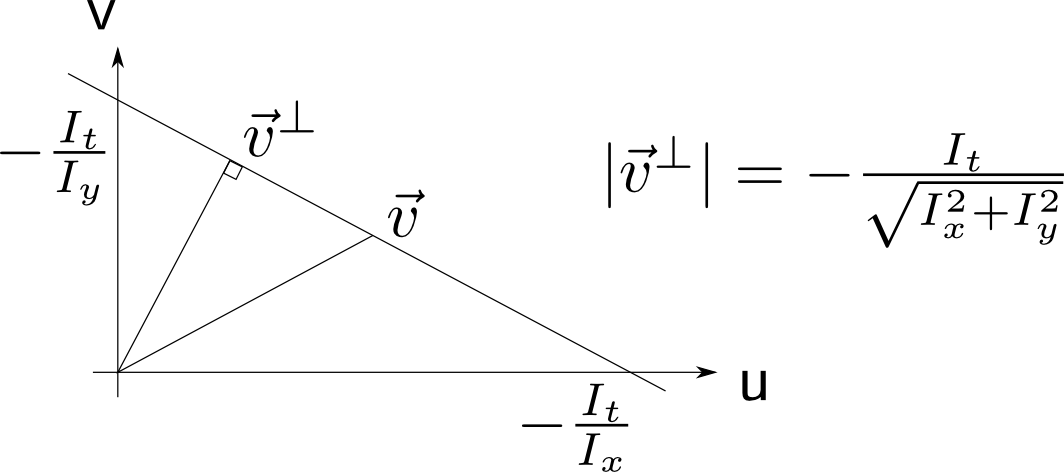
\includegraphics[scale=0.4]{figureOpticalConstraint.png}
\caption{Contrainte du flux optique}
\end{figure}

\subsection{Analyses et suivi}
Cette étape a pour objectif la comparaison des zones d'intérêt et la reconnaissance de celles-ci comme consistantes.

Le suivi de cibles s'apparente à l'étiquetage d'objets comme uniques, au travers du flux vidéo, c'est la reconnaissance des cibles dans la séquence d'image. \\

Pour en arriver au suivi d'objets, on aura dû effectuer la localisation de cibles par segmentation et leur représentation par extraction de traits d'intérêt.
Les images y ont été réduites aux traits essentiels permettant une caractérisation relativement robuste des cibles. 

Le procédé de suivi sera alors caractérisé par les opérations de \emph{filtrage} et d'\emph{association de données}.  \\

Le processus de reconnaissance est opéré à partir des descripteurs précédemment extraits dont on aura estimé l'évolution suivant notamment leur dynamique. Il y a donc la création d'une prédiction à partir de laquelle sera évaluée la correspondance avec l'observation de l'image au moment présent. 

\paragraph{Évaluation et filtrage}
Parmi les filtres les plus courant, il y a le filtre de Kalman et les filtres à particules.

Le filtre de Kalman est décrit comme ayant de bons résultats pour des systèmes à dynamique linéaire ou unimodale, typiquement gaussienne. L'approche par filtres à particules semble plus indiquée dans le cadre du suivi de cibles, car la prédiction de l'état courant doit prendre en compte toutes les alternatives possibles simultanément, en ce sens, la dynamique du système y est multimodale.
Le filtre \textit{condensation} sera décrit plus en détails dans le chapitre "Méthodes implémentées". \\  

Il existe de nombreuses façon d'évaluer la correspondance de données. 
Pour évaluer la correspondance, on compare les données dans une zone probable et on retient comme potentiellement correspondant les données pour lesquels on obtient la différence minimale.
 
Parmi les méthodes les plus connues, pouvant faire office de fonctions de mérite ou de corrélation: 
La distance de Mahalanobis et la distance euclidienne. 
Du fait de la simplicité d'implémentation pour un résultat satisfaisant, le calcul de la distance euclidienne a été utilisé.

\subsubsection{Distance euclidienne}
La correspondance par calcul de la distance euclidienne entre $2$ pixels n'est rien d'autre que la racine carrée de la somme du carré des différences en niveau de gris dans une zone $n*n$ autour des $2$ pixels.

$$ \sqrt{\sum_{i=0}^{n}\sum_{j=0}^{n}(a_{i,j} - b_{i,j})^2} $$


\pagebreak
%%%%%%%%%%%%%%%%%%%%%%%%%%%%%%%%%%%%%%%
\section{SURF}

%===================================================================================
\subsection{Speeded Up Robust Features}
%===================================================================================
Le \textit{Speeded Up Robust Features} (SURF) est un algorithme de \textit{détection de caractéristique} présenté par des chercheurs de l'\textit{\'Ecole Polytechnique Fédérale} de Zurich et de l'\textit{Université Catholique de Louvain} pour la première fois en 2006\footnote{Herbert Bay, Tinne Tuytelaars et Luc Van Gool, "\textit{SURF: Speeded Up Robust Features}", dans 9th \textit{European Conference on Computer Vision}, Graz, Autriche, 7-13 mai 2006}, puis dans une version révisée en 2008\footnote{Herbert Bay, Andreas Ess, Tinne Tuytelaars et Luc Van Gool, "\textit{SURF: Speeded Up Robust Features}", \textit{Computer Vision and Image Understanding}, vol. 110, no 3, 2008, p. 346-359}.
L'objectif de l'algorithme est de rechercher les correspondances entre objets ou scènes présentes dans deux ou plusieurs images distinctes mises en confrontation deux à deux. Il comporte 3 phases. 
\\Dans un premier temps, l'algorithme recherche des points intéressants de l'image, comme par exemple les points de bords ou les jointures en «T». Ces points doivent être faciles à déterminer, c'est-à-dire, que leurs caractéristiques sont telles que leur détermination doit être toujours reproductible sans ambigüité. \\ 
Ensuite, l'algorithme associe à chaque point d'intérêt un vecteur caractéristique qui représente un descripteur. Celui-ci, doit être distinct et surtout robuste par rapport au bruit, aux erreurs d'individuation et aux déformations géométriques et photométriques. \\
Enfin,  l'algorithme compare les descripteurs des deux images. Cette comparaison se base généralement sur la distance entre les vecteurs, par exemple, la distance euclidienne.

%===================================================================================
\subsection{Recherche des points d'intérêt}
%===================================================================================
\subsubsection{Image Intégrale}
L'efficacité de l'algorithme SURF est dû principalement à l'utilisation d'une représentation intermédiaire de l'image connue sous le nom d'\textit{image intégrale}.
\\L'image intégrale est une image numérique qui est calculée rapidement à partir de l'image originale. On l'utilise pour accélérer le calcul de chaque zone rectangulaire dont le sommet supérieur gauche est à l'origine de l'image. 
\\Proposée en 1984\footnote{Crow, Franklin (1984). "\textit{Summed-area tables for texture mapping}". SIGGRAPH '84: \textit{Proceedings of the 11th annual conference on Computer graphics and interactive techniques}: 207–212} comme méthode d'\textit{infographie}, c'est en 2001 qu'elle a été reformulée par la méthode de Viola et Jones\footnote{Paul Viola et Michael Jones, \textit{Robust Real-time Object Detection} IJCV 2001}, dans le cadre de la \textit{vision par ordinateur}.
\begin{figure}[ht]
\centering
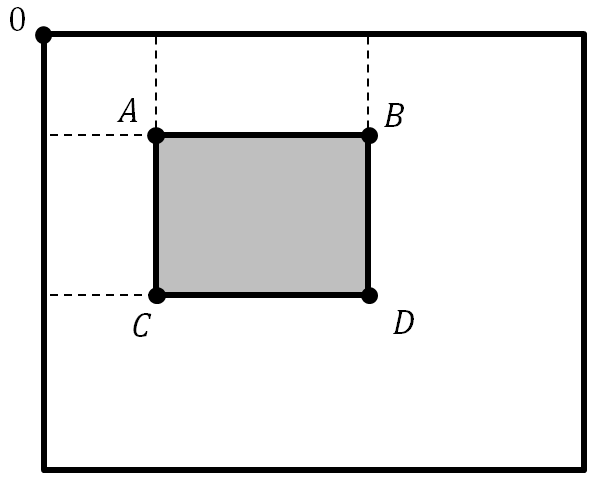
\includegraphics[scale=0.3]{figure1.png}
\caption{Calcul d'une aire en utilisant une image intégrale.}
\label{fig1}
\end{figure}
\\Étant donné une image $I$ en \textit{input} et un point de coordonnées $(x,y)$, l'image intégrale $I(x,y)$ est calculée en prenant la somme des valeurs de l'intensité des pixels compris entre le point et l'origine. Formellement, la formule est :
$$I_{\Sigma}(x,y)=\sum_{i=0}^{i\leq x} \sum_{j=0}^{j\leq y} I(x,y)$$
En utilisant l'image intégrale, le calcul de la somme des intensités d'une région rectangulaire quelconque se réduit à quatre opérations. En effet, si l'on considère un rectangle définit par les sommets $A$, $B$, $C$, $D$ (figure~\ref{fig1}), la somme qui donne la valeur de l'image intégrale vaut :
$$ \Sigma = A+D-(C+B)$$
où $A$, $B$, $C$, $D$ sont les intégrales correspondantes aux coordonnées des sommets. Ce calcul est invariant par rapport aux dimensions de la zone considéré et SURF utilise cette propriété pour effectuer de façon efficace la \textit{convolution} lorsque les dimensions des filtres appliqués à l'image varient.
\\La convolution est l'outil qui permet la construction de filtres linéaires ou de filtres de déplacements invariants. L'équation de convolution, notée $g(x)$, de la séquence $f(x)$ avec une fonction $h(x)$ est :
$$g(x)=f(x)\ast h(x)=\sum_{\forall k}h(x-k)f(k)$$
$f(x)$ est la fonction d'origine, $g(x)$ est la fonction qui résulte de la convolution et $h(x)$ est le noyau de convolution.
\begin{figure}[ht]
\centering
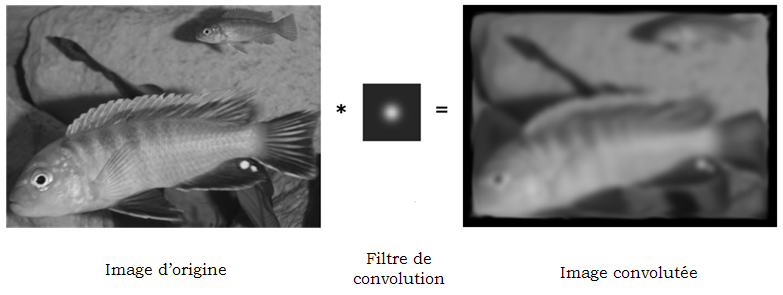
\includegraphics[scale=0.3]{figure2.png}
\caption{Exemple de convolution 2D.}
\label{fig2}
\end{figure}
%===================================================================================
\subsubsection{Points d'intérêt basés sur la matrice Hessienne}
Le \textit{détecteur} SURF se base sur le déterminant de la \textit{matrice hessienne}. Pour comprendre son fonctionnement, on considère une fonction continue $f$ de deux variables telle que :
$$f:x,y\mapsto f(x,y)$$
La matrice hessienne, $H$, est la matrice des dérivées partielles de la fonction $f$ :
$$
H(f(x,y))=
\begin{bmatrix}
\frac {\partial^2 f(x,y)}{\partial x^2} &\frac {\partial^2 f(x,y)}{\partial x \partial y} \\
\frac {\partial^2 f(x,y)}{\partial x \partial y} &\frac {\partial^2 f(x,y)}{\partial y^2}
\end{bmatrix}
$$
Le déterminant de cette matrice est calculé de la façon suivante :
$$\left|H(f(x,y))\right|=\frac{\partial^2 f(x,y)}{\partial x^2} \frac{\partial^2 f(x,y)}{\partial y^2} - \left(\frac{\partial^2 f(x,y)}{\partial x \partial y}\right)^2 $$
Ce déterminant est utilisé pour trouver le maximum et le minimum de la fonction à travers le test du hessien des dérivées secondes. En appliquant le test, il est alors possible de savoir si un point $(x,y)$ est un extremum local pour la fonction $f$.\\
Les dérivées partielles secondes sont calculées en utilisant un \textit{filtre gaussien normalisé du second ordre}, qui permet une analyse à plusieurs échelles et dans l'espace. Grâce à ce calcul, il est possible de déterminer les points du filtre en $x$, $y$ et $xy$ et de calculer les quatre termes de la matrice. L'utilisation de la gaussienne permet en outre, de faire varier l'effet de lissage durant la phase de convolution de façon à permettre le calcul du déterminant à différentes échelles.
\\\'Etant donné que la gaussienne est une fonction \textit{isotrope} (c'est-à-dire à symétrie circulaire), la convolution avec le point est invariant à la rotation. Il est alors possible de calculer la matrice hessienne comme fonction du point $\mathsf{x}=(x,y)$ et de l'échelle $\sigma$.
$$
H(\mathsf{x},\sigma)=
\begin{bmatrix}
L_{xx}(\mathsf{x},\sigma) &L_{xy}(\mathsf{x},\sigma)\\
L_{xy}(\mathsf{x},\sigma) &L_{yy}(\mathsf{x},\sigma)
\end{bmatrix}
$$
Ici, $L_{xx}(\mathsf{x},\sigma)$ se réfère à la convolution de la dérivée gaussienne de second ordre $\frac{\partial^2 g(\sigma)}{\partial x^2}$ avec l'image $I$ au point $\mathsf{x}=(x,y)$ et de façon analogue on définit $L_{yy}(\mathsf{x},\sigma)$ et $L_{xy}(\mathsf{x},\sigma)$. Ces dérivées sont connues comme LoG (\textit{Laplacian of Gaussian}).
\begin{figure}[ht]
\centering
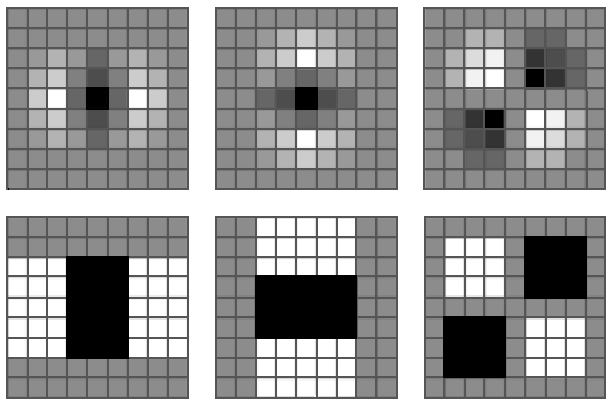
\includegraphics[scale=0.3]{figure3.png}
\caption{Approximation du laplacien de gaussienne.}
\label{fig3}
\end{figure}
\\L'approximation des LoG se fait à travers les approximations des points respectifs. La figure~\ref{fig3} montre les similitudes entre les filtres originaux et ceux obtenus par approximation et discrétisation.
\\Une amélioration des performances peut s'obtenir en utilisant conjointement les filtres avec les images intégrales. Et pour une approximation du determinant de la hessienne plus précise, on utilise une approximation de gaussienne.
$$\det(H_{approx})=D_{xx}D_{yy}-(0.9D_{xy})^2$$
La perte de precision est amplement compensée par une augmentation d'efficacité et de vitesse.
\\La recherche des maximum locaux dans l'espace à travers les différentes échelles conduit à l'identification des points d'intérêt de l'image.
%===================================================================================
\subsubsection{Espace d'échelle}
La théorie des \textit{espaces d'échelle} (\textit{Scale space theory}) est un model qui est apparu progressivement\footnote{Witkin, A. P. "\textit{Scale-space filtering}", Proc. 8th Int. Joint Conf. Art. Intell., Karlsruhe, Germany,1019–1022, 1983} \footnote{Koenderink, Jan "\textit{The structure of images}", Biological Cybernetics, 50:363–370, 1984} \footnote{Florack, Luc, "\textit{Image Structure}", Kluwer Academic Publishers, 1997} \footnote{Romeny, Bart ter Haar, "\textit{Front-End Vision and Multi-Scale Image Analysis}", Kluwer Academic Publishers, 2003} dans le domaine de la vision par ordinateur, pour prendre en compte la nature résolument multi-échelles des données images. L'espace d'échelle (\textit{scale-space}) est donc une fonction qui est utilisée pour trouver des points à travers toute les échelles possibles de l'image. Cette fonction est implémentée comme une pyramide dans laquelle l'image en \textit{input} est iterativement convolutée avec un point gaussien, et à maintes reprises redimensionnée. 
\\\'Etant donné que les coûts de computation des points utilisés par SURF sont invariants par rapport à leurs dimensions, l'espace d'échelle est créé en appliquant des points toujours plus grands à l'image originale. Ceci permet aux différents niveaux de la pyramide de l'espace d'échelle d'être calculés simultanément dans une éventuelle implémentation \textit{multithread}.
\begin{figure}[ht]
\centering
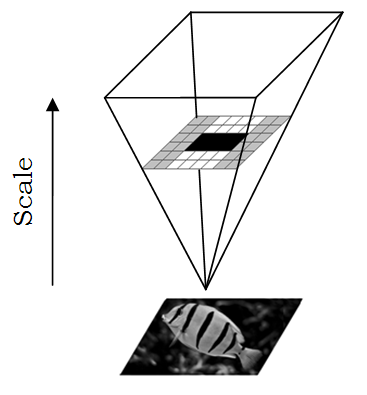
\includegraphics[scale=0.3]{figure4.png}
\caption{Pyramide du filtre.}
\label{fig4}
\end{figure}
\\La figure~\ref{fig4} montre l'espace d'échelle utilisée par SURF. Seul le filtre varie, contrairement à l'image originale qui reste invariante.
\\ Dans SURF, le niveau le plus bas d'espace d'échelle est obtenu en appliquant des filtre $9\times9$ comme ceux de la figure~\ref{fig3}. Ces filtres correspondent à une gaussienne avec un écart type $\sigma$ qui vaut 1,2. Les niveaux successifs sont obtenus en incrémentant les filtres de bases et en conservant les proportions (figure~\ref{fig5}).
\begin{figure}[ht]
\centering
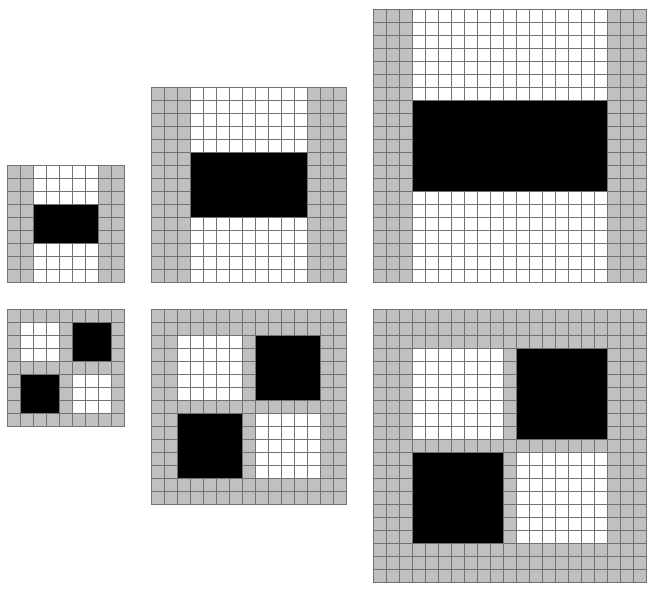
\includegraphics[scale=0.3]{figure5.png}
\caption{Structure du filtre.}
\label{fig5}
\end{figure}
\\\'Etant donnée que les proportions sont conservées lorsque les dimensions des filtres et l'échelle augmentent, il est possible de  calculer la formule suivante :
$$\sigma_{approx}=CurrentFilterSize.\frac{BaseFilterScale}{BaseFilterSize}=CurrentFilterSize.\frac{1,2}{9}$$
%===================================================================================
\subsubsection{Localisation des points d'intérêts}
Le processus de détermination de l'échelle qui permet de trouver les points d'intérêt d'une image se divise en 3 partie. Dans un premier temps, on applique un filtre avec un seuil pour faire en sorte d'éliminer les valeurs trop petites (en augmentant ce seuil le nombre de points diminue).
\\Successivement, on applique une \textit{suppression non-maximale} pour pouvoir trouver un ensemble de points candidats. Chaque pixel de l'espace d'échelle est confronté avec ses 26 points voisins, y compris les 8 points de l'échelle native et les 9 de chaque échelle supérieure et inférieure (figure~\ref{fig6}). Le pixel est un maximum s'il a une valeur supérieure à celle des pixels qui l'entourent à son échelle, à l'échelle supérieure et à celle inférieure. Si cette valeur est inférieure, il s'agit d'un minimum. \`A cette étape on dispose donc d'un ensemble de points d'intérêt filtrés qui sont soit un minimum, soit un maximum dans l'espace d'échelle.
\begin{figure}[ht]
\centering
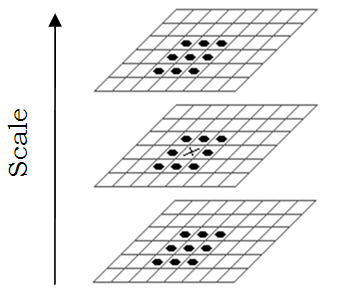
\includegraphics[scale=0.3]{figure6.png}
\caption{Suppression non maximale.}
\label{fig6}
\end{figure}
\\L'étape finale consiste à interpoler les données dans le but de localiser de façon précise les points d'intérêt (les maximums).
%===================================================================================
\subsection{Descripteur des points d'intérêt}
%===================================================================================
Les \textit{descripteurs} SURF décrivent la distribution des intensités des pixels autours des points d'intérêt sélectionnés. Ce résultat est possible grâce à l'utilisation des \textit{filtres Haar}, qui servent à déterminer les gradients dans les directions $x$ et $y$.
\begin{figure}[ht]
\centering

\includegraphics[scale=0.3]{figure7.png}
\caption{\textit{Haar Wavelets}.}
\label{fig7}
\end{figure}
\\Le filtre à gauche de la figure~\ref{fig7} calcule la réponse dans la direction $x$, tandis que celui à droite effectue le calcul par rapport à $y$. Les poids valent 1 pour les régions noires et -1 pour les régions blanches. Quand ces filtres sont utilisés avec les images intégrales, seules 6 opérations sont nécessaires pour obtenir un résultat. 
\\L'extraction des  descripteurs se divise en 2 phases. Tout d'abord pour chaque point d'intérêt on détermine une orientation, ensuite on construit une fenêtre centrée sur le point, dont la dimension dépend de l'échelle à laquelle le point d'intérêt a été trouvé. \`A partir de cette zone, et avec l'utilisation conjointe des filtres Haar et de l'image intégrale, on extrait un vecteur de 64 composantes.
%===================================================================================
\subsubsection{Composantes du descripteur}
Le premier pas dans l'extraction des descripteurs SURF consiste à construire une fenêtre carrée centrée au point d'intérêt. Cette fenêtre contient les pixels qui produiront le descripteur. Sa dimension est de $20\sigma$, avec $\sigma$ l'échelle à laquelle le point d'intérêt a été trouvé. La fenêtre est orientée de façon à ce qu'elle concorde à l'orientation du point.
\begin{figure}[ht]
\centering
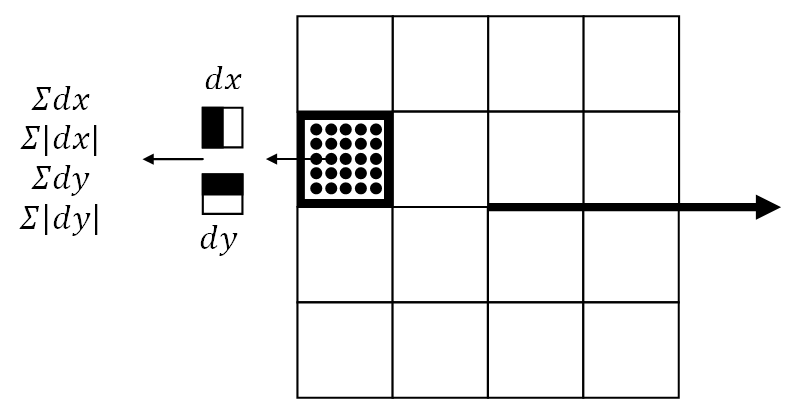
\includegraphics[scale=0.3]{figure8.png}
\caption{Composants du descripteur.}
\label{fig8}
\end{figure}
\\La fenêtre du descripteur est divisée en sous-régions  $4\times4$. \`A l'intérieur de chaque sous-région les filtres de Haar, de dimension $2\sigma$, sont appliqués sur 25 points uniformément distribués. Pour chaque région (pour les 25 points) on a : 
$$v_{sous-region}= \left[ \sum dx,\sum dy,\sum |dx|,\sum |dy|\right]$$
\`A la figure~\ref{fig8}, le carré à la bordure épaisse est une des 16 sous-régions et les points internes représentent les échantillons sur lesquelles est calculé le résultat donné par les \textit{Haar Wavelets}.

%%%%%%%%%%%%%%%%%%%%%%%%%%%%%%%%%%%%%%%%%%
\section{Exigences}
Suite à ce qui a été énoncé, il est intéressant de dégager quelques exigences auxquels se devrait de répondre un système de tracking robuste. 
\begin{itemize}
\item \textit{Faux positifs, faux négatifs et résistance à la pollution d'éléments parasites}, il convient de ne suivre que ce qui doit l'être.
\item \textit{Fiabilité quand à une possible occlusion}, il est fort probable qu'à un moment ou l'autre, la cible sera occulté par un autre élément et réapparaîtra ensuite. Le tracking doit alors rester consistant.
\item \textit{Souplesse du tracking}, celui-ci doit pouvoir suivre des éléments aux vitesses variables.
\item \textit{Stabilité}, malgré tout, le suivi de la cible doit perdurer.
\end{itemize}

\pagebreak
%%%%%%%%%%%%%%%%%%%%%%%%%%%%%%%%%%%%%%%%%%
\chapter{Méthodes implémentées}

%----------------------------------------------------------------------------------------
%	Méthodes implémentées : Condensation
%----------------------------------------------------------------------------------------
\section{Segmentation, traits d'intérêt et comparaison}
En liaison à l'implémentation de l'algorithme \textit{condensation}, différentes procédures, telles que décrites dans le chapitre précédent, ont été réalisées.\\

L'algorithme \textit{condensation}, qui effectue la principale tâche du suivi de cibles, reste ouvert sur les traitements annexes possibles quant au contexte dans lequel il s'effectue. 

Entre autres, les choix et les procédés d'extraction des traits d'intérêts, ainsi que la méthode d'estimation de la correspondance entre prédiction et observations, peuvent être réalisés de différentes façons.\\

L'extraction de l'avant-plan, la transformation en image binaire et la détection de contours ont été implémentées en vue de discerner les zones potentiellement intéressantes.

L'extraction de traits d'intérêts et l'estimation du mouvement (vitesse et direction) ont été utilisées pour établir les descripteurs de chaque cible.

La maximisation de la correspondance, c'est-à-dire la recherche de la différence minimale, a majoritairement été assurée par le calcul de la distance euclidienne.\\

Les descriptions de ces procédures ont été explicité dans le chapitre précédent.


\section{Conditionnal Density Propagation}
\subsection{Introduction}

Vulgairement, l'algorithme disperse, suivant une certaine probabilité, une suite de particules autour d'un trait d'intérêt. 

La correspondance de chacune des particules avec les observations est évaluée et donne un poids. 

Il en résulte une pondération des particules qui vient, après ré-échantillonnage, affiner la prédiction pour l'étape suivante. 

Le ré-échantillonnage évince les particules à faible probabilité. 

Le processus récursif fait converger les particules vers le trait de correspondance maximale.\\

Concrètement, afin de suivre un objet en mouvement au travers d'un flux vidéo, on doit être en mesure de déterminer à chaque \textit{frame} la position de la cible. 

C'est un processus d'anticipation sur le futur, où on peut soit évaluer toutes les possibilités, soit inférer à partir de ce qu'on connait et réduire au maximum le nombre de possibilités à tester. 

La détermination est rarement exacte car d'une part, la situation à évaluer est généralement d'une grande complexité et d'autre part, le processus de détermination s'appuie sur de nombreuses mesures, pour la plupart instables. 

La déformation de la cible, son occlusion, des changements de luminosité, etc, sont autant de mesures dont la propension à varier aléatoirement contribue à la génération de \emph{bruit} dans la détermination de la cible.\\  

Un des objectifs de la méthode est d'approcher l'hypothétique détermination réelle qui aurait été obtenue aux moyens de mesures idéales. 

Autrement dit, la méthode devrait être en mesure de mettre en exergue le tout ou une partie de la cible comme n'appartenant pas au \emph{bruit}.\\

Le processus de détermination se base sur un mouvement cyclique. Partant d'un modèle donné dont la paramétrisation est issue d'observations antérieures, on consolide ce modèle en évaluant sa pertinence à l'état présent. Ce mouvement conduit à une prédiction sur l'état probable à l'étape suivante.\\ 

On distingue alors deux phases, la \textit{prédiction} et l'\textit{observation}. 
\begin{description}
\item [La prédiction] est basée sur un modèle affiné par les informations passées, en vue d'\textit{estimer} l'état a posteriori.
\item [L'observation] ou phase de mesure, est la récolte d'informations sur l'état courant du système en vue de \textit{corriger} la prédiction basée sur les mesures précédentes.\\
\end{description}
 
\begin{figure}[H]

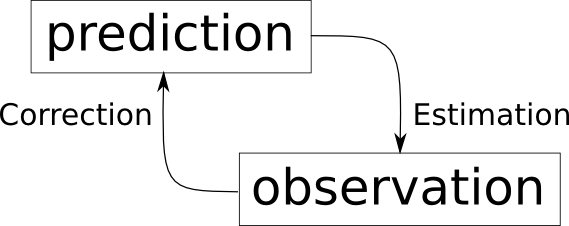
\includegraphics[scale=0.5]{figurePredictionObservationCycle.png}
\centering
\caption{Cycle de prédiction - observation}
\end{figure}

\subsection{Notation}
\begin{description}
\item[L'image] globale au moment $k$ est notée $I_k$, son historique est l'ensemble $$I_{0:n}=\{I_k, k=0,\cdots,n\}$$
\item[L'objet] est la zone d'intérêt dans l'image dont on souhaite faire le suivi.
\item[l'état de l'objet] $\mathbf{x}$ au temps $t$ est noté $\mathbf{x}_t$ et son historique est l'ensemble $$\mathcal{X}_{0:t} = \{\mathbf{x}_0,...,\mathbf{x}_t\}$$
\item[Les observations] sont l'ensemble des \textit{features} (traits \textit{invariants}) aussi dit \emph{descripteur} ou vecteur de \textit{features} $\mathbf{z}_t$ et son historique $$ \mathcal{Z}_{0:t}=\{\mathbf{z}_0,...,\mathbf{z}_t\}$$
\item[La dynamique] stochastique de l'objet est entièrement donnée par $$P(\mathbf{x}_t|\mathbf{x}_{t-1})$$ (processus Markovien)
\item[Les invariants] sont les caractéristiques locales de luminance ou géométrique.
\end{description}

\subsection{Filtre à particules et Monte-Carlo}
L'algorithme \textit{condensation} appartient à la classe des filtres particulaires. 

Les filtres à particules, aussi appelé méthodes  de Monte-Carlo séquentielles, s'appuient sur des méthodes statistiques. Ils ont pour dessein l'estimation de l'état d'un système donné et qui n'est pas toujours directement observable.
\textit{Condensation} contient en plus une approche bayésienne dans son processus d'approximation de l'état à calculer.\\

L'intérêt des méthodes de Monte-Carlo survient lorsque les méthodes numériques nécessitent une discrétisation de l'espace du problème. Cette discrétisation a pour effet d'augmenter la complexité de la recherche de solutions. Les techniques et optimisations probabilistes simplifient cette recherche de solutions.

Les méthodes Monte-Carlo dites séquentielles sont fondées sur des simulations numériques facilitant aussi le calcul d'une distribution a posteriori. La discrétisation de l'espace des possibles est alors comme borné par une densité donnée.\\

Les composantes du filtre particulaire apposé au suivi d'objets sont:
\begin{enumerate}
\item La séquence d'image $I_0,\cdots,I_n$ à des instants $t_0<\cdots<t_n$ est une suite d'observations $\mathbf{z}_t$ appartenant à la séquence observée $ \mathcal{Z}_{0:t}=\{\mathbf{z}_0,...,\mathbf{z}_t\}$.
\item[] L'image entière est définie comme un système complexe dont l'évolution se manifeste de façon discrète au travers de la séquence vidéo.
\item La cible que l'on souhaite suivre est un état caché $\mathbf{x}_k$ duquel on peut postuler l'existence:
	\begin{itemize}
	\item d'une suite d'états $\mathbf{x}_1,\cdots,\mathbf{x}_n$ corrélée à une suite d'instants $t_0,\cdots,t_n$ 
	\item d'un état initial $\mathbf{x}_0$ muni d'une \textit{loi initiale}  $P(\mathbf{x}_0)$
	\item d'une \textit{loi de transition} ou d'\textit{évolution} d'un état $\mathbf{x}_{t-1}$ à $\mathbf{x}_{t}$, soit $P(\mathbf{x}_t|\mathbf{x}_{t-1})$
\end{itemize}
\item Une loi d'\textit{observation} $P(\mathbf{z}_{t+\tau}|\mathbf{x}_{t+\tau})$\\
\end{enumerate}

\begin{figure}[H]
\centering
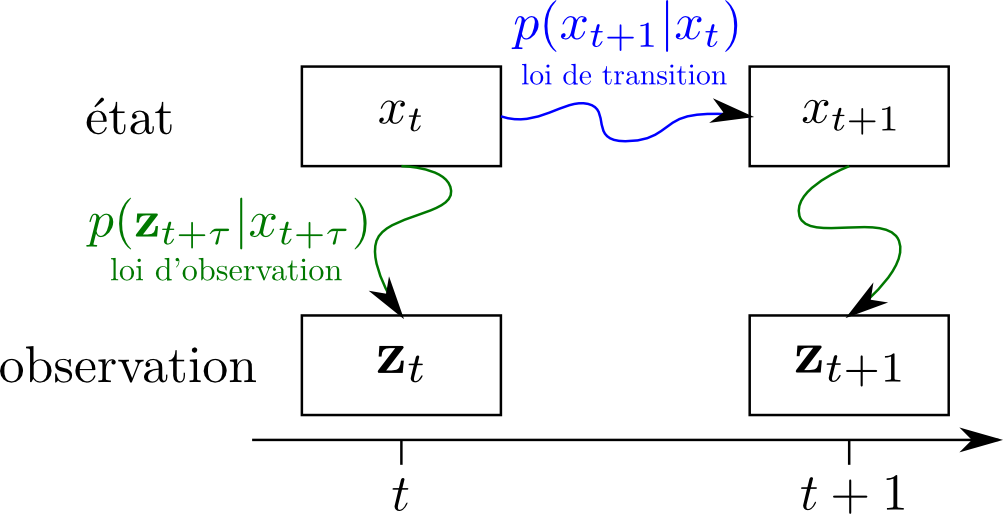
\includegraphics[scale=0.5]{figureCondensationLois.png}
\end{figure}

À partir de ces postulats, il est possible de:
\begin{enumerate}
\item \textit{Estimer}, c'est-à-dire établir une \textit{loi de proposition} caractérisant la relation entre l'état de l'objet conditionnellement aux observations: $P(\mathbf{x}_t|\mathcal{Z}_{1:t})$
\item \textit{Filtrer}, soit connaître $P(\mathbf{x}_t|\mathcal{Z}_{1:t+\tau})$
\item \textit{Prédire}, soit déterminer $P(\mathbf{x}_t|\mathcal{Z}_{1:t-1})$\\
\end{enumerate}

L'algorithme \textit{condensation} propose donc d'approcher l'état du système a posteriori en utilisant une connaissance a priori de celui-ci.
 
À partir d'une connaissance a priori du système et d'observations desquelles peut être caractérisée la variabilité statistique des données $z$ d'une image relativement à l'état de l'objet $x$, la distribution a posteriori $P(\mathcal{X}_{0:t}|\mathcal{Z}_{1:t})$ peut être estimée pour chaque $x_t$ étant donné $z_t$ au temps $t$.\\

\subsection{Chaîne Markov}
L'hypothèse est faite que la dynamique des objets forme une chaîne de Markov telle que $$P(\mathbf{x}_{t}|\mathcal{X}_{0:t})=P(\mathbf{x}_t|\mathbf{x}_{t-1})$$
Le processus stochastique possède la propriété de Markov si la distribution conditionnelle de probabilités des états futurs, étant donné les états passés et l'état présent, ne dépend que de l'état présent. 
On parle d'absence de mémoire au sein du processus.
La dynamique future de l'objet ne dépend pas de la séquence passée, mais uniquement de son état au temps présent.


\subsection{Approche bayésienne}
Le théorème de Bayes est:

$$P(A_i|B) = \frac{P(B | A_i) P(A_i)}{\sum_j P(B|A_j)P(A_j)}$$

où transposée à la problématique du suivi de cible, elle s'écrit:

$$P(\mathcal{X}_{0:t}|\mathcal{Z}_{1:t}) =  \frac{P(\mathcal{Z}_{1:t}|\mathcal{X}_{0:t})P(\mathcal{X}_{0:t})}{\int_{\mathcal{X}_{t+1}}P(\mathcal{Z}_{1:t}|\mathcal{X}_{0:t})P(\mathcal{X}_{0:t})d_{\mathcal{X}_{0:t}}}$$\\

Cette formulation, que le coût computationnel rend impraticable comme telle, devra être résolue de façon récursive. 
La formulation récursive fait apparaître la notion de vraisemblance et d'a priori sur l'état prédit.
$$P(\mathcal{X}_{0:t+1}|\mathcal{Z}_{1:t+1}) = P(\mathcal{X}_{0:t}|\mathcal{Z}_{1:t})\frac{P(\mathbf{z}_{t+1}|\mathbf{x}_{t+1})P(\mathbf{x}_{t+1}|\mathbf{x}_{t})}{P(\mathbf{z}_{t+1}|\mathcal{Z}_{1:t})}$$
où,
\begin{itemize}
\item[] la vraisemblance est donnée comme $P(\mathbf{z}_{t+1}|\mathbf{x}_{t+1})$
\item[] l'a priori est $P(\mathbf{x}_{t+1}|\mathbf{x}_{t})$\\
\end{itemize}

La densité a posteriori est exprimable comme fonction de l'\textit{observation} (évaluation de vraisemblance) et de la loi de \textit{transition}.

\subsection{Observation}
Les observations $\mathbf{z}_t$ sont indépendantes entre-elles et vis-à-vis du processus dynamique:
$$P(\mathcal{Z}_{1:t-1},\mathbf{x}_t|\mathcal{X}_{0:t-1}) = P(\mathbf{x}_t|\mathcal{X}_{0:t-1})\prod_{t=1}^{t-1} P(\mathbf{z}_t|\mathbf{x}_t)$$
ce qui se réduit, considérant la condition mutuelle d'indépendance des observations, en
$$P(\mathcal{Z}_{1:t}|\mathcal{X}_{0:t}) = \prod_{i=1}^{t} P(\mathbf{z}_i|\mathbf{x}_i)$$
Le processus d'observation est alors défini en spécifiant la densité conditionnelle $P(\mathbf{z}_t|\mathbf{x}_t)$ pour chaque instant $t$

\subsection{Propagation}
\`{A} partir des observations, la densité conditionnelle de l'état au moment $t$ est $P_t(\mathbf{x}_t) \equiv P(\mathbf{x}_t|\mathcal{Z}_ {1:t})$. Elle représente toute l'information de l'état pouvant être déduite de l'entièreté du flux de données.\\
Selon le théorème de Bayes, on déduit la règle de propagation de la densité de l'état dans le temps comme  
$$P(\mathbf{x}_{t}|\mathcal{Z}_{t}) = k_t P(\mathbf{z}_t|\mathbf{x}_t)P(\mathbf{x}_t|\mathcal{Z}_{1:t-1})$$
où $k$ représente une constante de normalisation ne dépendant pas de $\mathbf{x}_t$.\\
La densité \textit{a priori} $P(\mathbf{x}_t|\mathcal{Z}_{1:t-1})$ est une prédiction issue de la densité \textit{a posteriori} $P(\mathbf{x}_{t-1}|\mathcal{Z}_{1:t-1})$ à laquelle a été surimposé un pas de temps du modèle dynamique (temporalité indépendante du flux vidéo).
La règle de propagation est alors $$P(\mathbf{x}_t|\mathbf{z}_t) = kP(\mathbf{z}_t|\mathbf{x}_t)P(\mathbf{x}_t)$$
Pour atteindre cette densité \textit{a priori} tout en évitant un coût computationnel conséquent, celle-ci est approchée de façon récursive par échantillonnage pondéré.\\

\subsection{Algorithme}

L'hypothèse du processus markovien et l'approche bayésienne posées, on défini récursivement l'estimation du système comme:
$$\mathtt{Est}(t) = P(\mathbf{z}_{t}|\mathbf{x}_{t})*P(\mathbf{x}_{t}|\mathbf{x}_{t-1})*\mathtt{Est}(t-1)$$

L'approximation récursive se déroule suivant le canevas:
\begin{center}
\begin{tabular}{ c c c c c } 
\cellcolor[gray]{0.9} Prédiction & $\rightarrow$ & \cellcolor[gray]{0.9} Mesure & $\rightarrow$ & \cellcolor[gray]{0.9} Échantillonnage \\  
\end{tabular} 
\end{center}

\begin{figure}[hbtp]
\centering
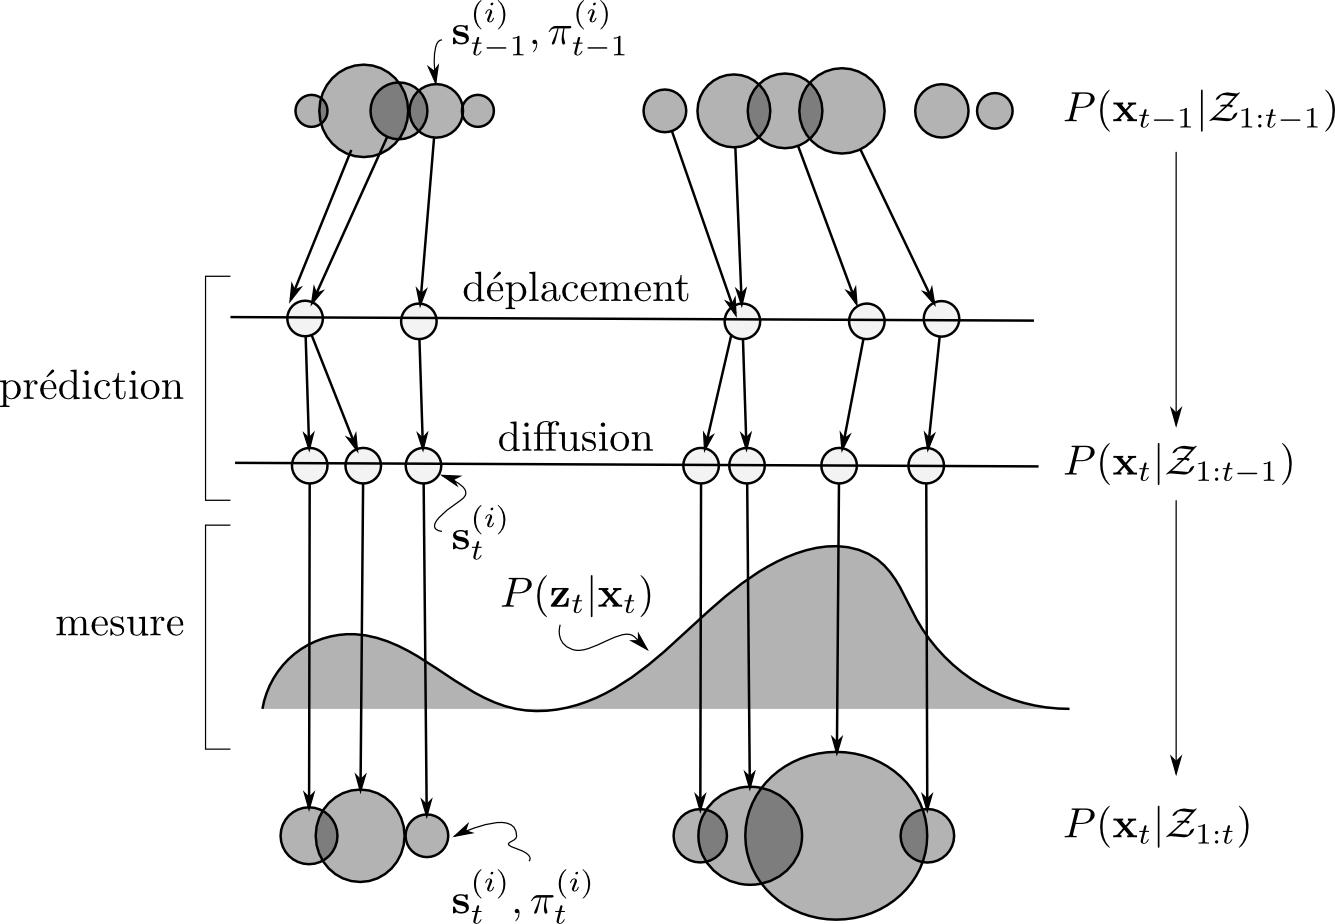
\includegraphics[scale=0.45]{figureCondensationAlgo.png}
\caption{Visualisation d'un pas de l'algorithme}
\end{figure}


\subsubsection{Prédiction}
La prédiction de la position d'une nouvelle particule $\mathbf{s'}_{t}^{(k)}$ est obtenue à partir de la densité a priori $P(\mathbf{x}_{t}|\mathbf{x}_{t-1})$ 

où 
\begin{itemize}
\item[] $P(\mathbf{x}_{t}|\mathbf{x}_{t-1} = \mathbf{s}_{t-1}^{(k)})$, pour $k = 1,\cdots,N$ 
\item[] $\mathbf{s}_{t-1}^{(k)}$ est issu du précédent échantillonnage.
\end{itemize}

\subsubsection{Mesure}

La pondération des particules déterminant la probabilité $\pi_t$ est obtenue à partir de la loi d'observation $P(\mathbf{z}_{t+}|\mathbf{x}_{t})$ 

où
\begin{itemize}
\item[] $P(\mathbf{z}_{t+}|\mathbf{x}_{t} = \mathbf{s'}_{t}^{(k)})$, pour $k = 1,\cdots,N$
\item[] $\mathbf{s'}_{t}^{(k)}$ est issu de la prédiction
\end{itemize}
   

\subsubsection{Échantillonnage}
Il s'agit de retrouver un objet $\mathbf{x}$ de densité \textit{a priori} $P(\mathbf{x})$ en utilisant les données observées $\mathbf{z}$ d'une image.
La densité \textit{a posteriori} est calculée récursivement par échantillonnage pondéré dont le canevas est le suivant:
\begin{enumerate}
\item Soit un vecteur $S_{t-1}$ de $N$ échantillons pris sur l'image $I_{t-1}$,
$$S_{t-1}=\{ \mathbf{s}_{t-1}^{(i)}, \pi_{t-1}^{(i)}, i=1,\cdots,N\}$$
\item[] Initialement, les poids $\pi_0^{(i)}$ valent $\frac{1}{N}$ 
\item $S_t$ est obtenu:
\item[]\verb+for+ $k=1$ à $N$,
\begin{enumerate}
\item[] On sélectionne un échantillon $\mathbf{s}_t^{(k)}$ du vecteur $S_{t-1}$ relativement à son poids $\pi_{t-1}^{(i)}$ issu la probabilité $\pi_{t-1}$
\end{enumerate}
\end{enumerate} 

On obtient un vecteur $$S_{t}=\{ \mathbf{s}_{t}^{(i)}, \pi_{t}^{(i)}, i=1,\cdots,N\}$$ où les faibles particules ont été évincées.




\chapter{Résultats expérimentaux}

%----------------------------------------------------------------------------------------
%	Résultats expérimentaux
%----------------------------------------------------------------------------------------

\section{Différences}
La réalisation présentée à l'issue du projet se différencie de l'approche proposée par les auteurs M. Isard et B. Andrew, en un certain nombre de points:
\begin{enumerate}
\item \textit{Condensation} est présenté avec l'utilisation de \textit{splines} pour descripteurs \cite{condIsard}. Dans ce travail, le choix a été fait de baser le suivi de cible sur des points robustes non mis en relation, à la manière d'un \textit{blob}.
\item La problématique du suivi de poissons à orienté l'implémentation vers une solution potentiellement multi-cibles.
\end{enumerate}


\section{Scénario de solution logicielle}
La trame de la solution esquissée par le présent travail se décrit comme suit:
\begin{enumerate}
	\item Détection de cible
	\begin{enumerate}
		\item Segmentation
		\item Sélection des points intéressants
		\item Mémorisation de la cible
	\end{enumerate}
	\item Suivi de cible
	\begin{enumerate}
		\item Identification des traits d'intérêt
		\begin{enumerate}
			\item Choix de candidats selon une distribution
			\item Élection du meilleur candidat: première passe et ré-échantillonnage
		\end{enumerate}
		\item Élimination des traits non robustes ou perdus\\
	\end{enumerate}
\end{enumerate}

L'application commence par segmenter l'image et y détecter des cibles, elle ne retournera à cette étape de segmentation que sous la condition d'avoir perdu un certain nombre de traits d'intérêt (seuil). 

Les cibles détectées, commence la phase de suivi dans laquelle la procédure cycle autant que possible.

De cette façon, l'application alterne des phases de recherche de cibles et de suivi de cibles.\\
 

\section{Le logiciel}

\subsection{Aperçu}
\begin{figure}[hbtp]
\centering
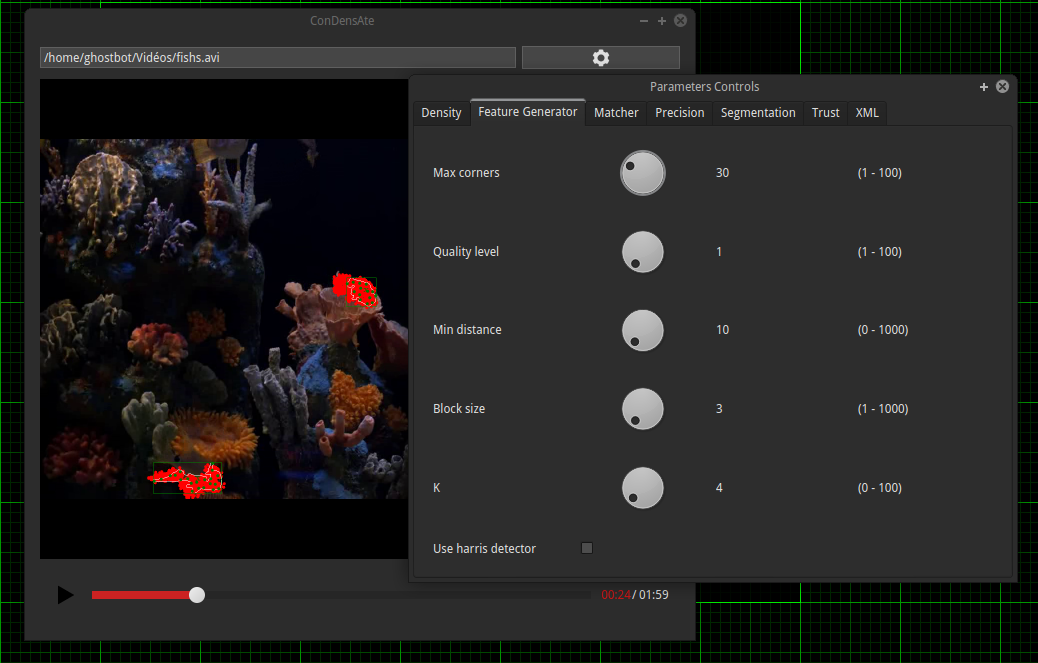
\includegraphics[scale=0.18]{screenshots/condensate3Cut.png}
\caption{aperçu de l'application ConDensAte}
\label{fig:aperçu}
\end{figure}

Le logiciel (\ref{fig:aperçu}) se compose d'une fenêtre principale au sein de laquelle peut être lu un flux vidéo provenant:
\begin{itemize}
\item d'un fichier.
\item d'une caméra locale ou usb.
\item d'une caméra en réseau (\ref{fig:camera}).
\end{itemize}

\begin{figure}[hbtp]
\centering
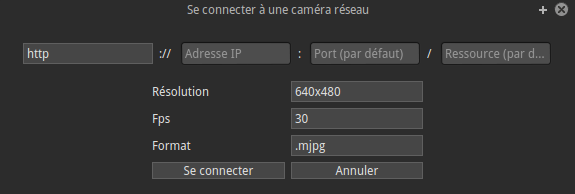
\includegraphics[scale=0.3]{screenshots/condensate4.png}
\caption{Connection à une caméra en réseau}
\label{fig:camera}
\end{figure}

En vue de répondre adéquatement, au diverses qualités et résolutions de vidéo, l'application propose de pouvoir paramétrer (\ref{fig:paramétrisation}) les différentes étapes de l'algorithme et de sauvegarder ces réglages au format XML.

\begin{figure}[H]
\centering
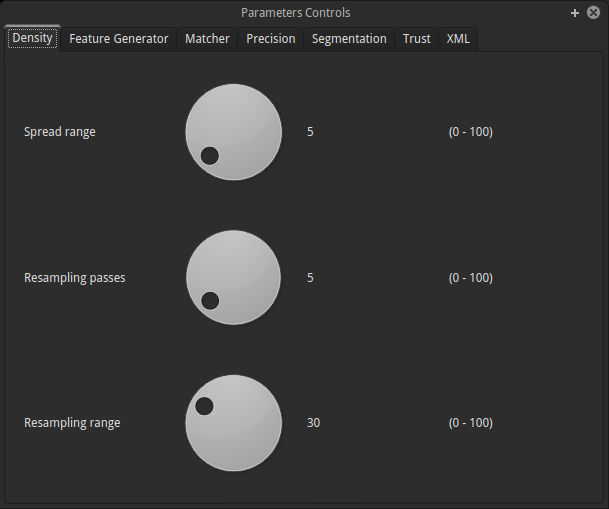
\includegraphics[scale=0.3]{screenshots/condensate5.png}
\caption{Paramétrisation}
\label{fig:paramétrisation}
\end{figure}

\pagebreak
\subsection{En action}

\begin{figure}[H]
\centering
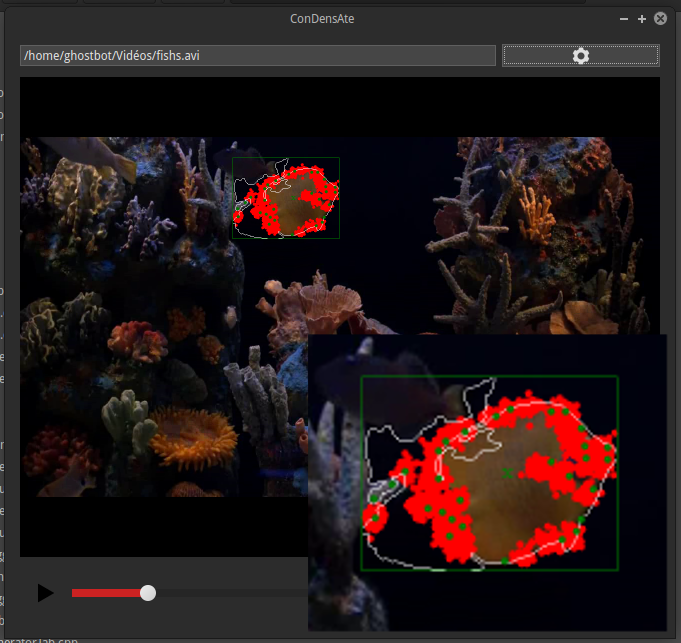
\includegraphics[scale=0.45]{screenshots/condensate24.png}
\caption{ConDensAte: Recherche de cibles}
\label{SegmentationCible}
\end{figure}

\paragraph{Détection de cibles}
L'application segmente l'image afin de cerner les régions potentiellement intéressantes (figure \ref{SegmentationCible} cadre vert). 

Cette segmentation, par différentiation des objets en mouvement et réalisée en utilisant un masque binaire, débouche sur une détection des contours de la cible éventuelle (figure \ref{SegmentationCible}, trait blanc). 

Au sein des contours, la recherche et l'extraction des traits d'intérêt, selon les recommandations de Shi et Tomasi \cite{o}, est effectuée. Un vecteur contenant les traits d'intérêt est alors créé.\\ 

\begin{figure}[H]
\centering
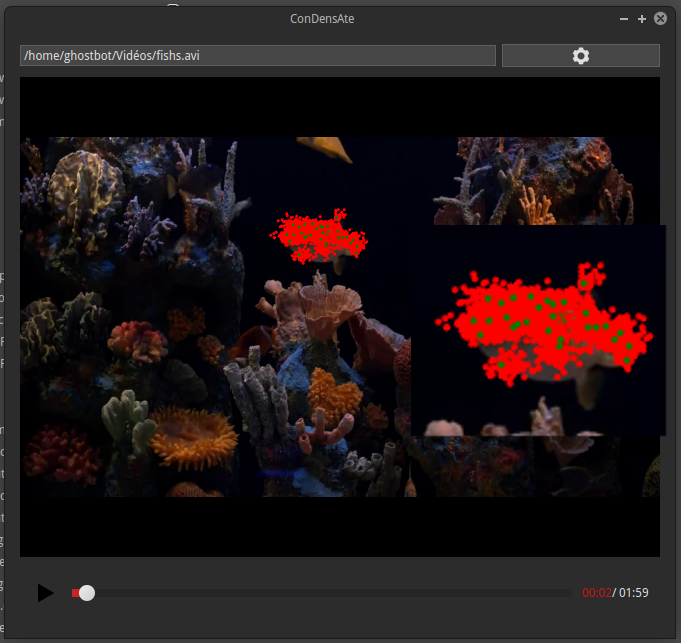
\includegraphics[scale=0.45]{screenshots/condensate14.png}
\caption{ConDensAte: Suivi de cibles}
\label{SuiviCible}
\end{figure}

\paragraph{Suivi de cibles}
À partir du vecteur de traits d'intérêts, pour chacun d'eux, l'application va établir des prédictions suivant une distribution donnée. 

Sur la figure \ref{SuiviCible}, les points rouges représentent les particules de la prédiction courante, les points verts les traits de la prédiction précédente qui ont satisfont au mieux la correspondance avec les traits d'intérêts initiaux.\\

\subsection{Code source}

L'application et le code source sont téléchargeables à l'adresse:
 \begin{center}
 \url{www.webresearch.be/fishtube}
 \end{center}   


\chapter{Conclusion et perspectives}

%----------------------------------------------------------------------------------------
%	Conclusion et perspectives
%----------------------------------------------------------------------------------------
L'application donne des résultats, dans une certaine mesure, satisfaisants. Mais l'implémentation telle que réalisée peut être largement améliorée.\\

Le algorithmes annexes (segmentation, vraisemblance, détection de \textit{features}) qui ont été utilisé ne sont pas forcément ceux qui donnent les résultats les plus précis.\\ 

Par exemple, il aurait été intéressant d'intégrer la puissance de l'algorithme SURF, ce qui aurait permis d'ajouter à la détection et au suivi de cibles, la reconnaissance du type de cibles selon des \textit{templates} données.

\bibliography{biblio}
\nocite{*}

\addcontentsline{toc}{chapter}{Bibliographie}
\listoffigures
\end{document}
